% Template for ICASSP-2010 paper; to be used with:
%          mlspconf.sty  - ICASSP/ICIP LaTeX style file adapted for MLSP, and
%          IEEEbib.bst - IEEE bibliography style file.
% --------------------------------------------------------------------------
\documentclass{article}
\usepackage{amsmath,graphicx,02460}
\pagestyle{plain}
\usepackage{subcaption}
\usepackage{comment}
\usepackage{hyperref}
\usepackage{ulem}

\pagenumbering{gobble}

\toappear{Pablo Táboas Rivas. Master Thesis}


% Example definitions.
% --------------------
\def\x{{\mathbf x}}
\def\L{{\cal L}}

% Title.
% ------
\title{Bayesian inference solution for vibroacoustic parameters estimation}
%
% Single address.
% ---------------
\name{Pablo Táboas (s212556)}
%\address{Author Affiliation(s)}
\address{}
%
% For example:
% ------------
%\address{School\\
%	Department\\
%	Address}
%
% Two addresses (uncomment and modify for two-address case).
% ----------------------------------------------------------
%\twoauthors
%  {A. Author-one, B. Author-two\sthanks{Thanks to XYZ agency for funding.}}
%	{School A-B\\
%	Department A-B\\
%	Address A-B}
%  {C. Author-three, D. Author-four\sthanks{The fourth author performed the work
%	while at ...}}
%	{School C-D\\
%	Department C-D\\
%	Address C-D}
%
\begin{document}
%\ninept
%

\maketitle
%
\begin{abstract}
The difference between experimental results and analytical ones make the simulations differ from the measurements. By using bayesian inference, the goal is to  the uncertainty between the theoretical values of electroacoustics parameters in order to fit both approaches.  
\end{abstract}
%
\begin{keywords}
Speech separation, Deep learning, Denoising, Bayesian Inference
\end{keywords}
%
\section{Introduction}
\label{sec:intro}
Estimating the vibroacoustic parameters of a hearing aid is a complex task to solve since there are multiple physical properties related to the overall behaviour of the device. In order to fit the best the analytical and FEM response with the experimental data, the problem is split into stages starting from the most simple model possible and adding layers of complexity. The stage explained in this report corresponds to the first stage where just the material properties of the beam are estimated by using bayesian inference. 

\section{Related work}
\label{sec:format}


\section{Theoretical background}
% intro of the section
The main task of this report can be split into two main fields of knowledge. The problem to solve consist of estimating different material properties in order to fit different approaches with experimental results. In a first stage, an analytical solution was proposed and, afterward, a FEM one.

\subsection{Vibroacoustic theory (mobility)}
\label{sec:theory}
The setup used for this experiment consists of a flat beam excited in its center by a harmonic point source. Considering the length of the beam as \textit{L}, the excitation point will be in $l = L/2$. For the experiment, as explained in \autoref{sec:setup}, the acceleration of the beam when excited under a specific force will be measured. The result of this measure will be expressed in terms of mobility which defines the relationship between the velocity of the beam and the force applied.  Having this into account, the mobility at that point can be modeled as
\begin{equation}
    \underline{Y}_{l l}=\frac{-(0.25 \eta+i) l}{2 k l \sqrt{B m^{\prime}} } \frac{ \underline{N}(\underline{k}_{l l})}{\underline{D}(\underline{k}_{l l})},
\end{equation}

where $k_b$ is the bending wave number, B the bending stiffness and  $m'$ the mass per unit length. 

The parameters to be estimated in this work are the material properties: Youngs' modulus(E), Poison ratio() and density($\rho$)

\section{Experimental setup}
\label{sec:setup}
This first stage of the project consists in studying the frequency response of a flat beam. The such beam is excited by a shaker as shown in \autoref{fig:setupFlat} and the response is measured with an accelerometer (placed over the beam) and a force transducer (between the shaker and the beam). The accelerometer must be glued directly to the beam with bee wax. The mass of the accelerometer must be taken into account since the variation of the total mass can produce variations in the  performance of the experiment. \textbf{Check documentation about the acceleration weight}. 

\begin{figure}[h]
    \centering
    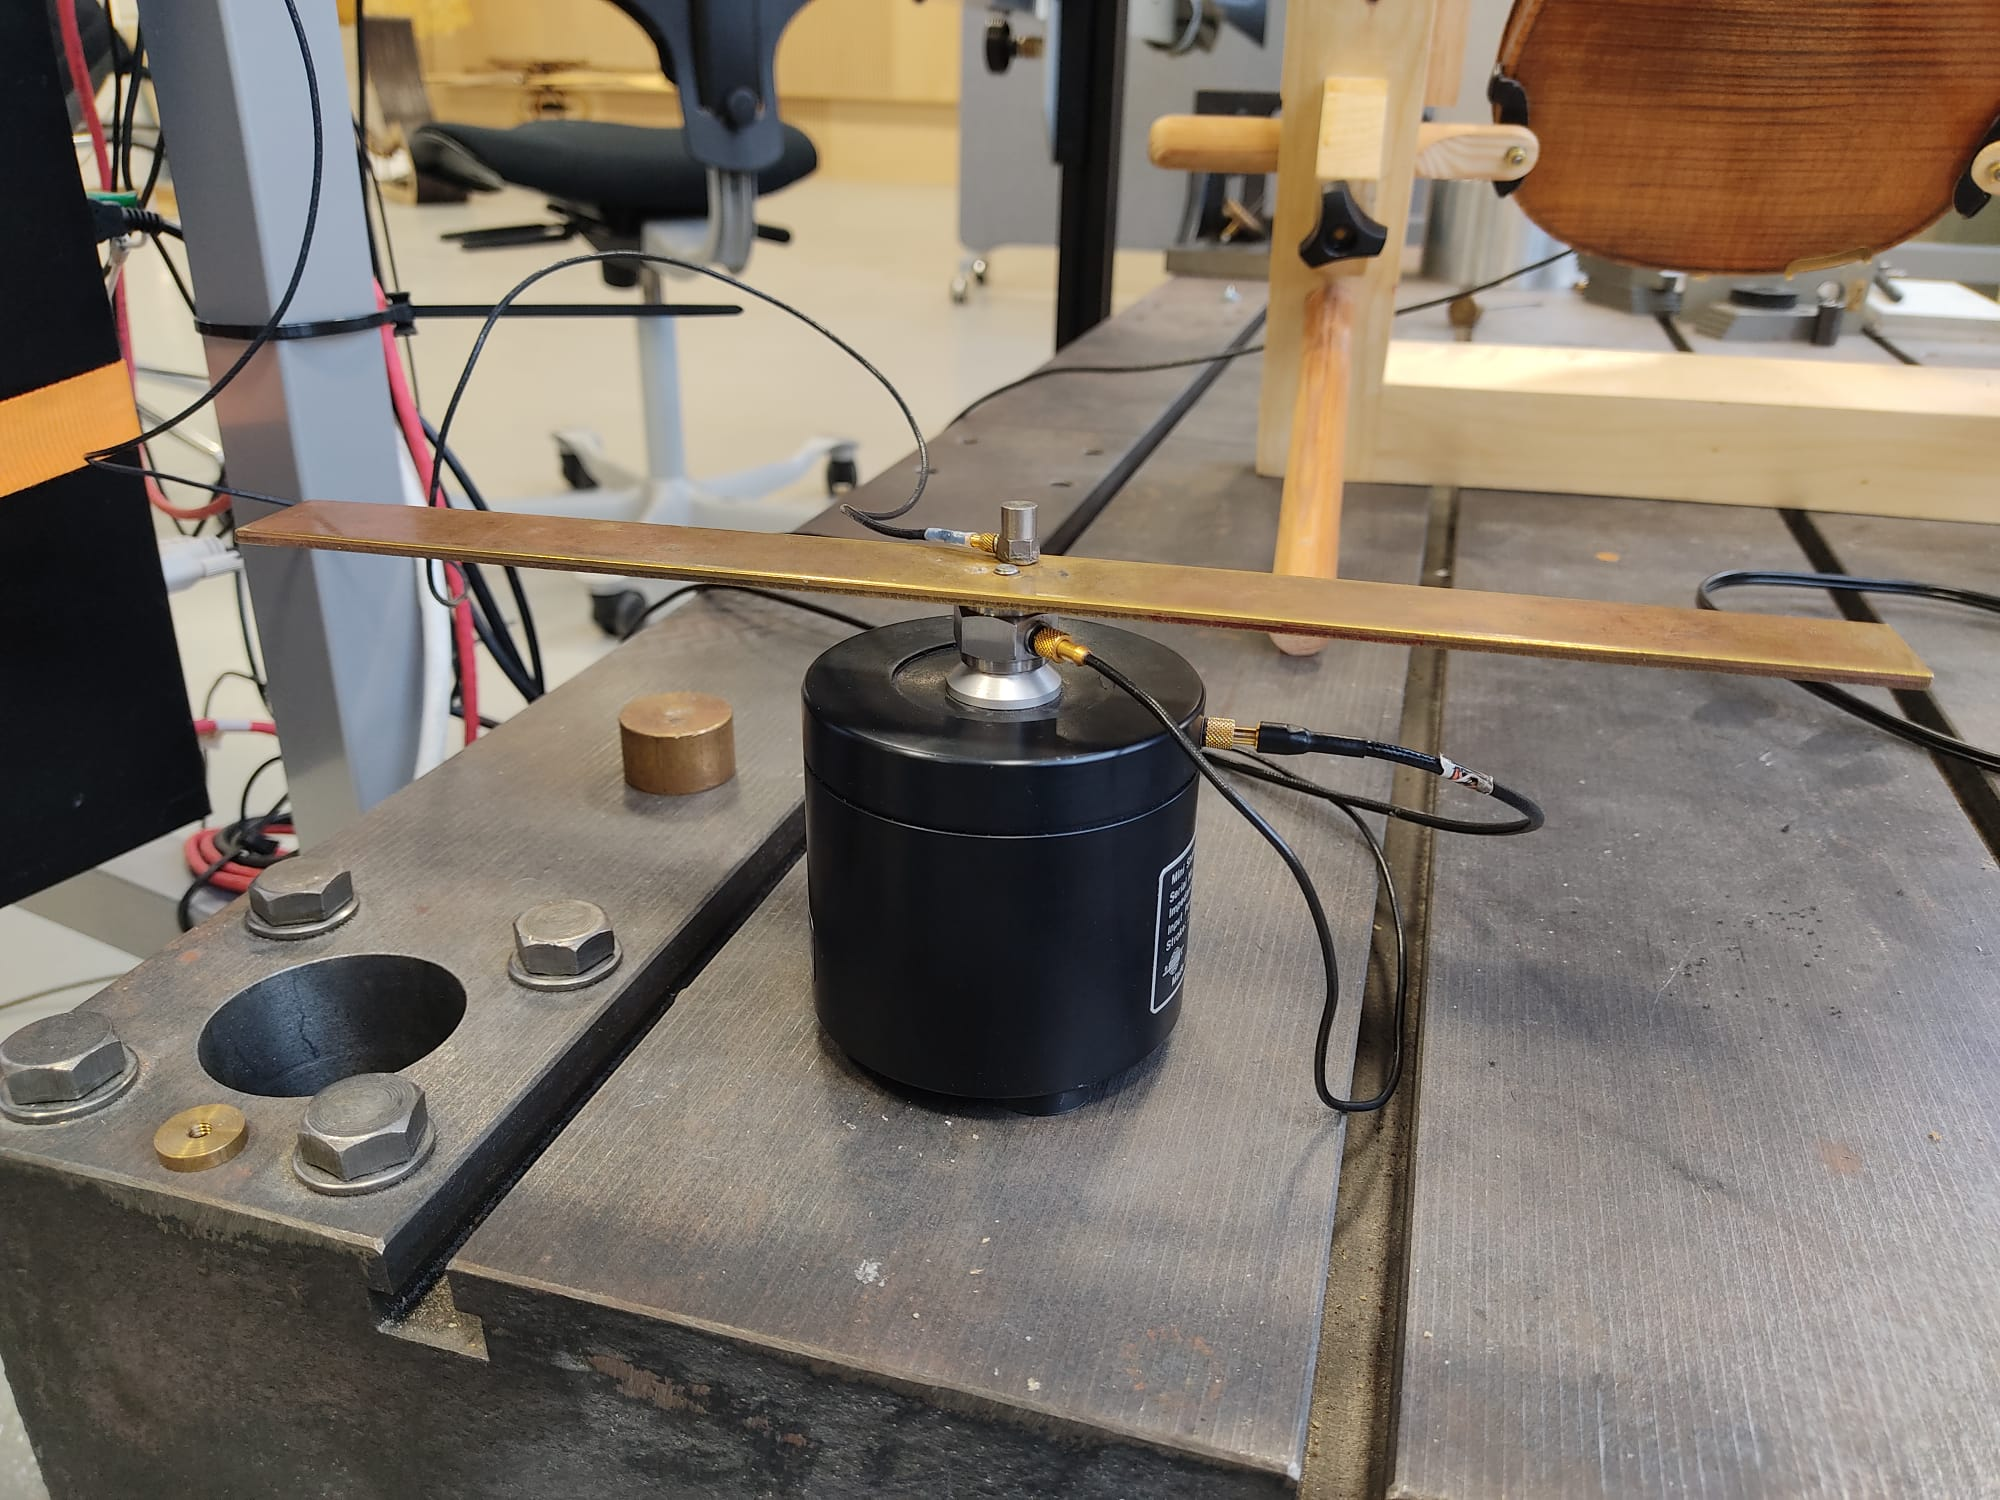
\includegraphics[width = 8cm]{pictures/expSetup.jpeg}
    \caption{Setup of the experiment with the brass beam. The accelerometer is placed over the beam and the force transducer between the shaker and the beam.}
    \label{fig:setupFlat}
\end{figure}

\subsection{Bayesian Modelling}
The estimation of de material properties will be studied following a bayesian inference process. Machine learning has traditionally two approaches: the statistical

\section{Experimental Results}
\label{sec:experimental_results}
In this section, we first provide our experimental results of the different approaches tested on 200 unseen samples of the LibriMix dataset. After, we show the results of the SVoice 2ch and 2+1ch approaches for different noise categories and noise intensities. 

Since the baselines from the mentioned publications were trained on much more data and higher computational resources, we use our own trained models from SVoice and DPRNN as a baseline to get comparable results (hereinafter referred to as SVoice 2ch and DPRNN 2ch). The baselines were trained with the same parameters and number of epochs.
\subsection{Comparison of Model Architectures}
\label{ssec:comparison_model_architectures}


The trend of the loss values for both models trained with SVoice is presented in figure \ref{fig:training_curve}. Since the loss values are decreasing during training, a learning of the target behavior can be detected. Whereas, in the beginning of training, the loss values of the two models are similar, in later epochs the 2+1 model  shows a better performance. It can also be observed that the curves of both models are not completely flattened at epoch 20, where we stopped the training due to high training times. This took around 48 hours per model. Hence, better results can be expected for training with more epochs. 

 The results are reported in Table \ref{tab:Results}. It can be seen that our 2+1ch approach outperforms the 2ch approach used in the publications for both SVoice and DPRNN by a sizable margin. Also, the models trained with the SVoice architecture outperform the results obtained by DPRNN on the new dataset. It should be mentioned that the obtained SI-SNRi values are much lower than the ones shown in \cite{Svoice} (15.2 and 13.9) since more training data and time were used by the authors.

 In addition, the described cascade approach for SVoice performs better than both the 2ch and the 2+1ch model. This approach requires a bigger model size and has a higher computational demand since two models are trained individually.  
 

The distribution of the SI-SNRi values  for the 200 samples used in testing for the mentioned approaches can be seen in the whisker plot in figure \ref{fig:Boxplot}.

\subsection{Generalizing in Different Noise Settings}
\label{ssec:comparison_model_architectures}

Next, we compared the performance of the SVoice 2ch and the proposed SVoice 2+1ch approach under different, unseen noise settings using the MS-SNSD dataset. The SI-SNRi results for the six chosen categories for an input SDR of 0 are presented in figure \ref{fig:NoiseCategories}. 

It can be seen that the 2+1ch approach has similar or slightly worse results than the 2ch approach for five of the six categories. A tendency, that one of the approaches works better on environmental noise (typing, nature, washing machine) or on human speaking background noise (cafe, babble, square) can not be observed. However, the 2+1ch model clearly outperforms the 2ch model for the \textit{Babble} noise category. This was observed for all tested noise intensities. Further investigations into the different noise samples showed that the \textit{Babble} noise is the most similar to the noise used in the WHAM! dataset, which might explain the good performance. Given the number of training samples and the variety of noise data our model was trained on, the 2+1ch model is not able to generalize well in different noise categories. 

In addition to adding unseen noise categories to the speaker files, we also varied the input SNR, which changes the intensity of the noise in relation to the speakers. The lower the SNR, the higher the noise intensity in the testing files. The results of the 2ch and 2+1ch models tested with files with noise from the category \textit{Café} with five different noise intensities are presented in figure \ref{fig:NoiseIntensities}. It can be seen that the 2+1ch model performs better than the 2ch model for low noise intensities, while it is worse for samples with high noise intensities. This behavior can be observed for all tested noise categories except for \textit{Babble} noise, where the 2+1ch model shows better results for the SI-SNRi for all five input SNR.

The performance of both models depends heavily on the noise intensity. In general, the lower the noise intensity, the higher the SI-SNRi. However, for both models, a flattening of the curve can be seen between SNR 0 and 5. This might be because the SNR for our training data set lies in this range, and therefore the models can not generalize well for higher noise intensities. 




% Below is an example of how to insert images. Delete the ``\vspace'' line,
% uncomment the preceding line ``\centerline...'' and replace ``imageX.ps''
% with a suitable PostScript file name.
% ---------------------------------------
% To start a new column (but not a new page) and help balance the last-page
% column length use \vfill\pagebreak.
% -------------------------------------------------------------------------
\vfill
\pagebreak


\section{Discussion and Future work}
\label{sec:discussion}
In this study, we evaluated the performance of various deep-learning models for speech separation in noisy environments. Unlike previous work, we trained models for both SVoice and DPRNN with an additional noise channel. For known noise, the obtained results for the models trained with an additional noise channel are better than those trained with the existing method, by a sizable gap. This suggests that explicitly modeling the noise in the training process can be beneficial for improving speech separation and denoising performance. For further analysis, our new training approach should be used with the same data and computational resources as in \cite{Svoice}, to find out if the baseline of an SI-SNRi of 15.2 can be outperformed.

However, for unknown noise conditions, the results of models with an additional noise channel were highly dependent on the specific noise category and intensity. Our models performed well for the noise category they were trained on (background speakers), but may not generalize well to other types of noise. We find that the 2+1ch model typically outperforms the 2ch model at low noise intensities. In further work, the training dataset should be created with a high variety of noise categories and input noise intensities and investigated if the new model is able to generalize better.

Additionally, we found that the SVoice model outperformed the DPRNN model on a new dataset (LibriMix), which confirms the results presented in \cite{Svoice}, indicating that SVoice may be a particularly effective approach. 

In addition, we also evaluated the effectiveness of multitask learning compared to a cascade approach. We find that the cascade approach performs slightly better than multi-task learning at the cost of increased computational demand. For this, two different models needed to be trained. In further work, a new training procedure or a new cascade model could be developed, which combines the two steps in a single model, so both tasks are improved simultaneously while training. 

Overall, these findings provide valuable insights into the capabilities and limitations of different approaches for training state-of-the-art models for speech separation in noisy environments.\\

The code of this project can be found in this github-repository: \url{https://github.com/AnnaGr-Git/DL_Denoising_SpeechSeparation}


% \section{REFERENCES}
% \label{sec:ref}

% List and number all bibliographical references at the end of the paper.  The references can be numbered in alphabetic order or in order of appearance in the document.  When referring to them in the text, type the corresponding reference number in square brackets as shown at the end of this sentence \cite{C2}.

% References should be produced using the bibtex program from suitable
% BiBTeX files (here: strings, refs, manuals). The IEEEbib.bst bibliography
% style file from IEEE produces unsorted bibliography list.
% -------------------------------------------------------------------------
\newpage
\bibliographystyle{IEEEbib}
\bibliography{refs}

\end{document}
